% Chapter Template

\chapter{Conclusion} % Main chapter title

\label{Chapter7} % Change X to a consecutive number; for referencing this chapter elsewhere, use \ref{ChapterX}

\lhead{Chapter 7. \emph{Conclusion}} % Change X to a consecutive number; this is for the header on each page - perhaps a shortened title

%----------------------------------------------------------------------------------------
%	SECTION 1
%----------------------------------------------------------------------------------------

\section{Summary of Important Points}
The aim of this thesis was to demonstrate how \ac{MRL} can be used to solve the symbol grounding problem in an unsupervised manner.

Through the course of the experiments shown in Chapters 4, 5 and 6, I have demonstrated that the joint representation of different data modalities solves the symbol grounding problem. This was shown to be the case as the correct image was generated for each utterance provided in \autoref{Chapter4}. Similarly, in \autoref{Chapter5} and \autoref{Chapter6}, I showed that images of objects could be generated from their decriptions and vice-versa even for unseen combinations of attributes. \textcolor{red}{Through these experiments, hypotheses 1, 3 and 6 were proven to be true. It is possible to solve the symbol grounding problem using \ac{MRL} with a \ac{MAE} for both images and sounds, and images and text regardless of whether the data is artificial or real.}

\textcolor{red}{In \autoref{Chapter4}, hypothesis 2 was proven, as \ac{MRL} was demonstrated to improve classification accuracy for the combined MNIST and UCU datasets.}

The learned representation has been demonstrated to fit some of the criteria layed out by Bengio et al. in \cite{repRev}. Particularly, the representation has been demonstrated to have Manifolds which can be manipulated through vector arithmetic to make predictable and meaningful changes in the output. For example, subtracting the representation of the word \textsc{red} from the representation of an image of a \textit{Red Triangle} and adding the representation of the word \textsc{Green} resulted in the generation of an image of a \textit{Green Triangle} in \autoref{Chapter5}.  \textcolor{red}{However, I am unable to accept the hypothesis 5 as the representation does not meet all of the criteria put forward by Bengio et al. The main issue with the learnt representation is its lack of smoothness - there are clearly gaps in the latent space which are unexplored due to contraints on the amount of training data available. The \ac{MAE} is unable to smoothly interpolate the meaning of the representation within these gaps as seen by the generation of incorrect images using vector arthmetic for some combinations of images and attributes (\autoref{fig:739_vectorArth} in \autoref{Chapter5}).}

In some datasets, such as MNIST and ArtS, it is possible to generate image prototypes for each class/word in the \ac{MAE}'s ``vocabulary''. For MNIST, this came in the form of prototypical versions of each digit and for ArtS, images of each colour, shape and size can be generated individually.

This is also possible for the ReShape dataset. However, due to the larger variability of training examples, the prototypes are very blurry. By using a class exemplar for each object, the \ac{MAE} was able to learn to generate non-blurry prototypes for each of the visual attributes.

I also demonstrated that \ac{MRL} can be used to generate accurate object descriptions of both real and artificial images. As well as that using \ac{MRL} can lead to improvements in classification accuracy as seen in \autoref{Chapter4} over unimodal baselines. However, this improvement comes at the cost of having worse performance when only a single modality is available.

In \autoref{Chapter5} and \autoref{Chapter6}, I showed that \ac{MRL} allows \acp{ANN} to generalise to unseen objects. The \ac{MAE} is able to correctly generate images of objects which do not appear in the training data by combining the representations of different words. This entire process relies on the \ac{MAE} having grounded the meaning of each word individually to its image-space equivalent. The best example of this was the generation of a \textsc{Big Red Donut}.

\section{Summary of contributions}
\textcolor{red}{In this thesis I have furthered the research of Ngiam et al. \cite{ngiam2011multimodal} and Silberer et al. \cite{silberer2014learning} into the miriad uses of \acp{MAE}. I have demonstrated how they can be used to solve the symbol grounding problem in an unsupervised manner for multiple datasets and data modalities. I have also demonstrated how \ac{MRL} can be used to enhance classification accuracy when multimodal data is available.}

\textcolor{red}{In carrying out this research I have produced two new datasets which can be used to explore object recognition, object attribute learning and language learning, namely the Arts and ReShape dataset. The script to generate the Arts dataset can be found here: https://bit.ly/30gX34s and the ReShape dataset can be downloaded here: https://bit.ly/3gn2YdO.}

\textcolor{red}{I have also developed a novel technique, which I have called vector arthmetic which allows for the exploration of the latent representation space of \acp{MAE}. Presented in \autoref{fig:vectorArthexmp} in \autoref{Chapter5}, my implementation of vector arthmetic builds off of the work of Mikolov et al. \cite{mikolov2013distributed, mikolov2013efficient, mikolov2013linguistic}. Vector arthmetic is a technique which takes the representations of objects and/or language and adds and subtracts them to generate new images or descriptions.} 

\textcolor{red}{The ability of my \ac{MAE} system to generate images and descriptions of unseen objects is, to my knowledge, entirely unique to it. Whilst Reed et al. \cite{reed2016generative} produced a GAN based system which was capable of generating images from unseen captions over a larger domain than that covered by either the Arts or ReShape datasets, it is only capable of this one directional process - it is not capable of generating decriptions of unseen objects. My \ac{MAE} based system performs a bidirectional process, generating both novel images and descriptions.}

\section{Conclusion}
\ac{MRL} has been shown to be a powerful technique and presents an area worthy of futher study. Whilst the findings of the experiments in this thesis are exciting, further work is needed to apply \ac{MRL} in a real world setting.

Unsupervised approaches to symbol grounding are vital to the development of robots for opperation in the real world. \ac{MRL} could form the foundation of a robotic cognitive system which can continue to learn throught its lifetime. Furthermore, the ability of the trained \acp{MAE} to generalise to unseen objects will make teaching robots about new objects quicker as it is not necessary to train the \ac{MAE} with every possible combination of visual attributes. Only a subset of attribute combinations needs to be learnt, from which other attribute combinations can be inferred as demonstrated in \autoref{Chapter5} when generating images of \textsc{Red Donuts}.

\textcolor{red}{Whilst Ngiam et al. \cite{ngiam2011multimodal}, were able to demonstrate how \acp{MAE} can be used to learn a joint representation of video and sound and how this can be used to enhance phoneme classification under noisy conditions, I was able to demonstrate that classification of MNIST Handwritten Digits and UCU Arabic Spoken Digits can be enhanced, even in noise free situations using the representation learnt by the \ac{MAE} in \autoref{Chapter4}. Ngiam et al. found that under noise free conditions, multimodal classification was lower than unimodal classification of phonemes for their dataset, this was not the case for the combined dataset used in this thesis where digit classification was enhanced by having access to multiple data sources.}

\textcolor{red}{The result found by Ngiam et al. \cite{ngiam2011multimodal} is somewhat surprising in light of the work done by Lawrence Baraslou \cite{barsalou2008grounded}. Baraslou expects that having multimodal data should enhance recognition (classification accuracy) by providing auxilory information. Barsalou explains that multimodality provides data redundancy, explaining the improvement in classification accuracy seen by Ngiam et al. in noisy conditions. Given the auxilory information provided by multimodality (the information which is unique to any one modality), I would expect that classification accucracy should be improved in all circumstances, not just noisy conditions. This is in line with the result I found in \autoref{Chapter4} where classifcation accuracy was improved by multimodality under noise free conditions. In future it would be worth while to explore whether this holds true for the combined MNIST and UCU dataset if noise were introduced.}

\section{Limitations}
\textcolor{red}{Whilst the research carried out in this thesis shows a promising avenue for future work, there are several limitations to the work carried out. In \autoref{Chapter5} a more extensive hyperparameter search could have lead to better image and description generation results. Most importantly, an embedding size of 296 was the largest tested due to time constraints. \aclp{ANN} are notorius for taking a long time to train, as such I was unable to explore larger embedding sizes.}

\textcolor{red}{When examining the quality of generated images, the lack of a quantitive measure beyond \ac{MSE} is a severe limitations. This limitation is found in other work \cite{reed2016generative, zhang2017stackgan, xu2018attngan, li2018video, mansimov2015generating}. However, the use of proxy scores like Inception score \cite{zhang2017stackgan}, would be useful for adding weight to the qualititive analysis of generated images.}

\textcolor{red}{Further to making use of Inception score, the use of human ratings, other than my own, via a service such as Amazon Mechanical Turk could also be used to rate the quality of generated images.}

\textcolor{red}{The large amount of blur in the images generated for the ReShape dataset made analysis of them difficult. Whilst this was alleviated by the introduction of the Exemplar training method, in general this is not the most desirable approach for dealing with this issue. The exemplar method requires that an exemplar for each object be computed. Whilst on a small dataset such as ReShape this is possible, it would not be practical for a robot in the wild. Computing a class exemplar involved finding the mean of the class, to do this on a robot would require keeping every instance of an object everytime it is seen. It would be possible to streamline this process by developing heuristics for determining the exemplar. However, it would be simpler to find an alternative method which does not require human intervention (the development of heurisitcs) such as the use of an adversarial cost function \cite{reed2016generative}.}

\section{Future Work}
The experiments layed out in the previous chapters have shown that \ac{MRL} using \acp{MAE} allows for the unsupervised learning of a grounded representation of images and language. How then, can this be used to improve robotic technologies?

I see many potential applications for \ac{MRL} within the field of \ac{HRI}. \autoref{fig:fsm} shows an example of how the \ac{MAE} can be included in a robotic system.


\begin{figure}
\centering
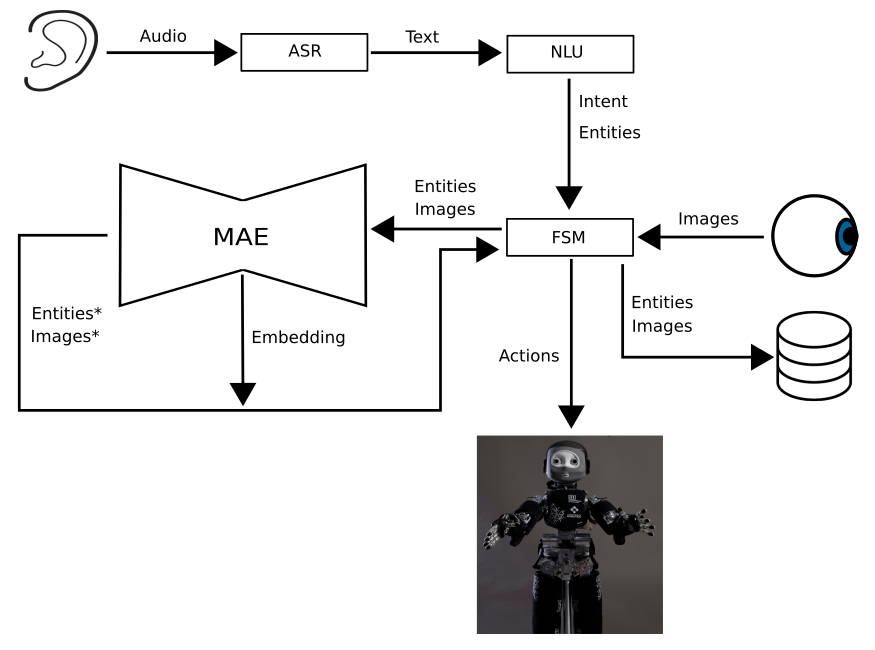
\includegraphics[width=\textwidth]{Figs/futureWork/fsm.png}
\caption{An example of how the \ac{MAE} can be used as part of a robotic system.}
\label{fig:fsm}
\end{figure}

Consider the scenario of a human interacting with a robot to teach it a set of objects and their visual attributes as well as the words used to describe the objects and their visual attributes. In a laboratory setting it is feasable to have only a single object in view at any given time. This is not true for real world scenarios. However, with the introduction of a \ac{FSM} controlled via a \ac{NLU} module, it is simple to use a \ac{MAE} trained with \ac{MRL} to discern which object is being referred to by the human. This is demonstrated in \autoref{fig:disamb}

\begin{figure}
\centering
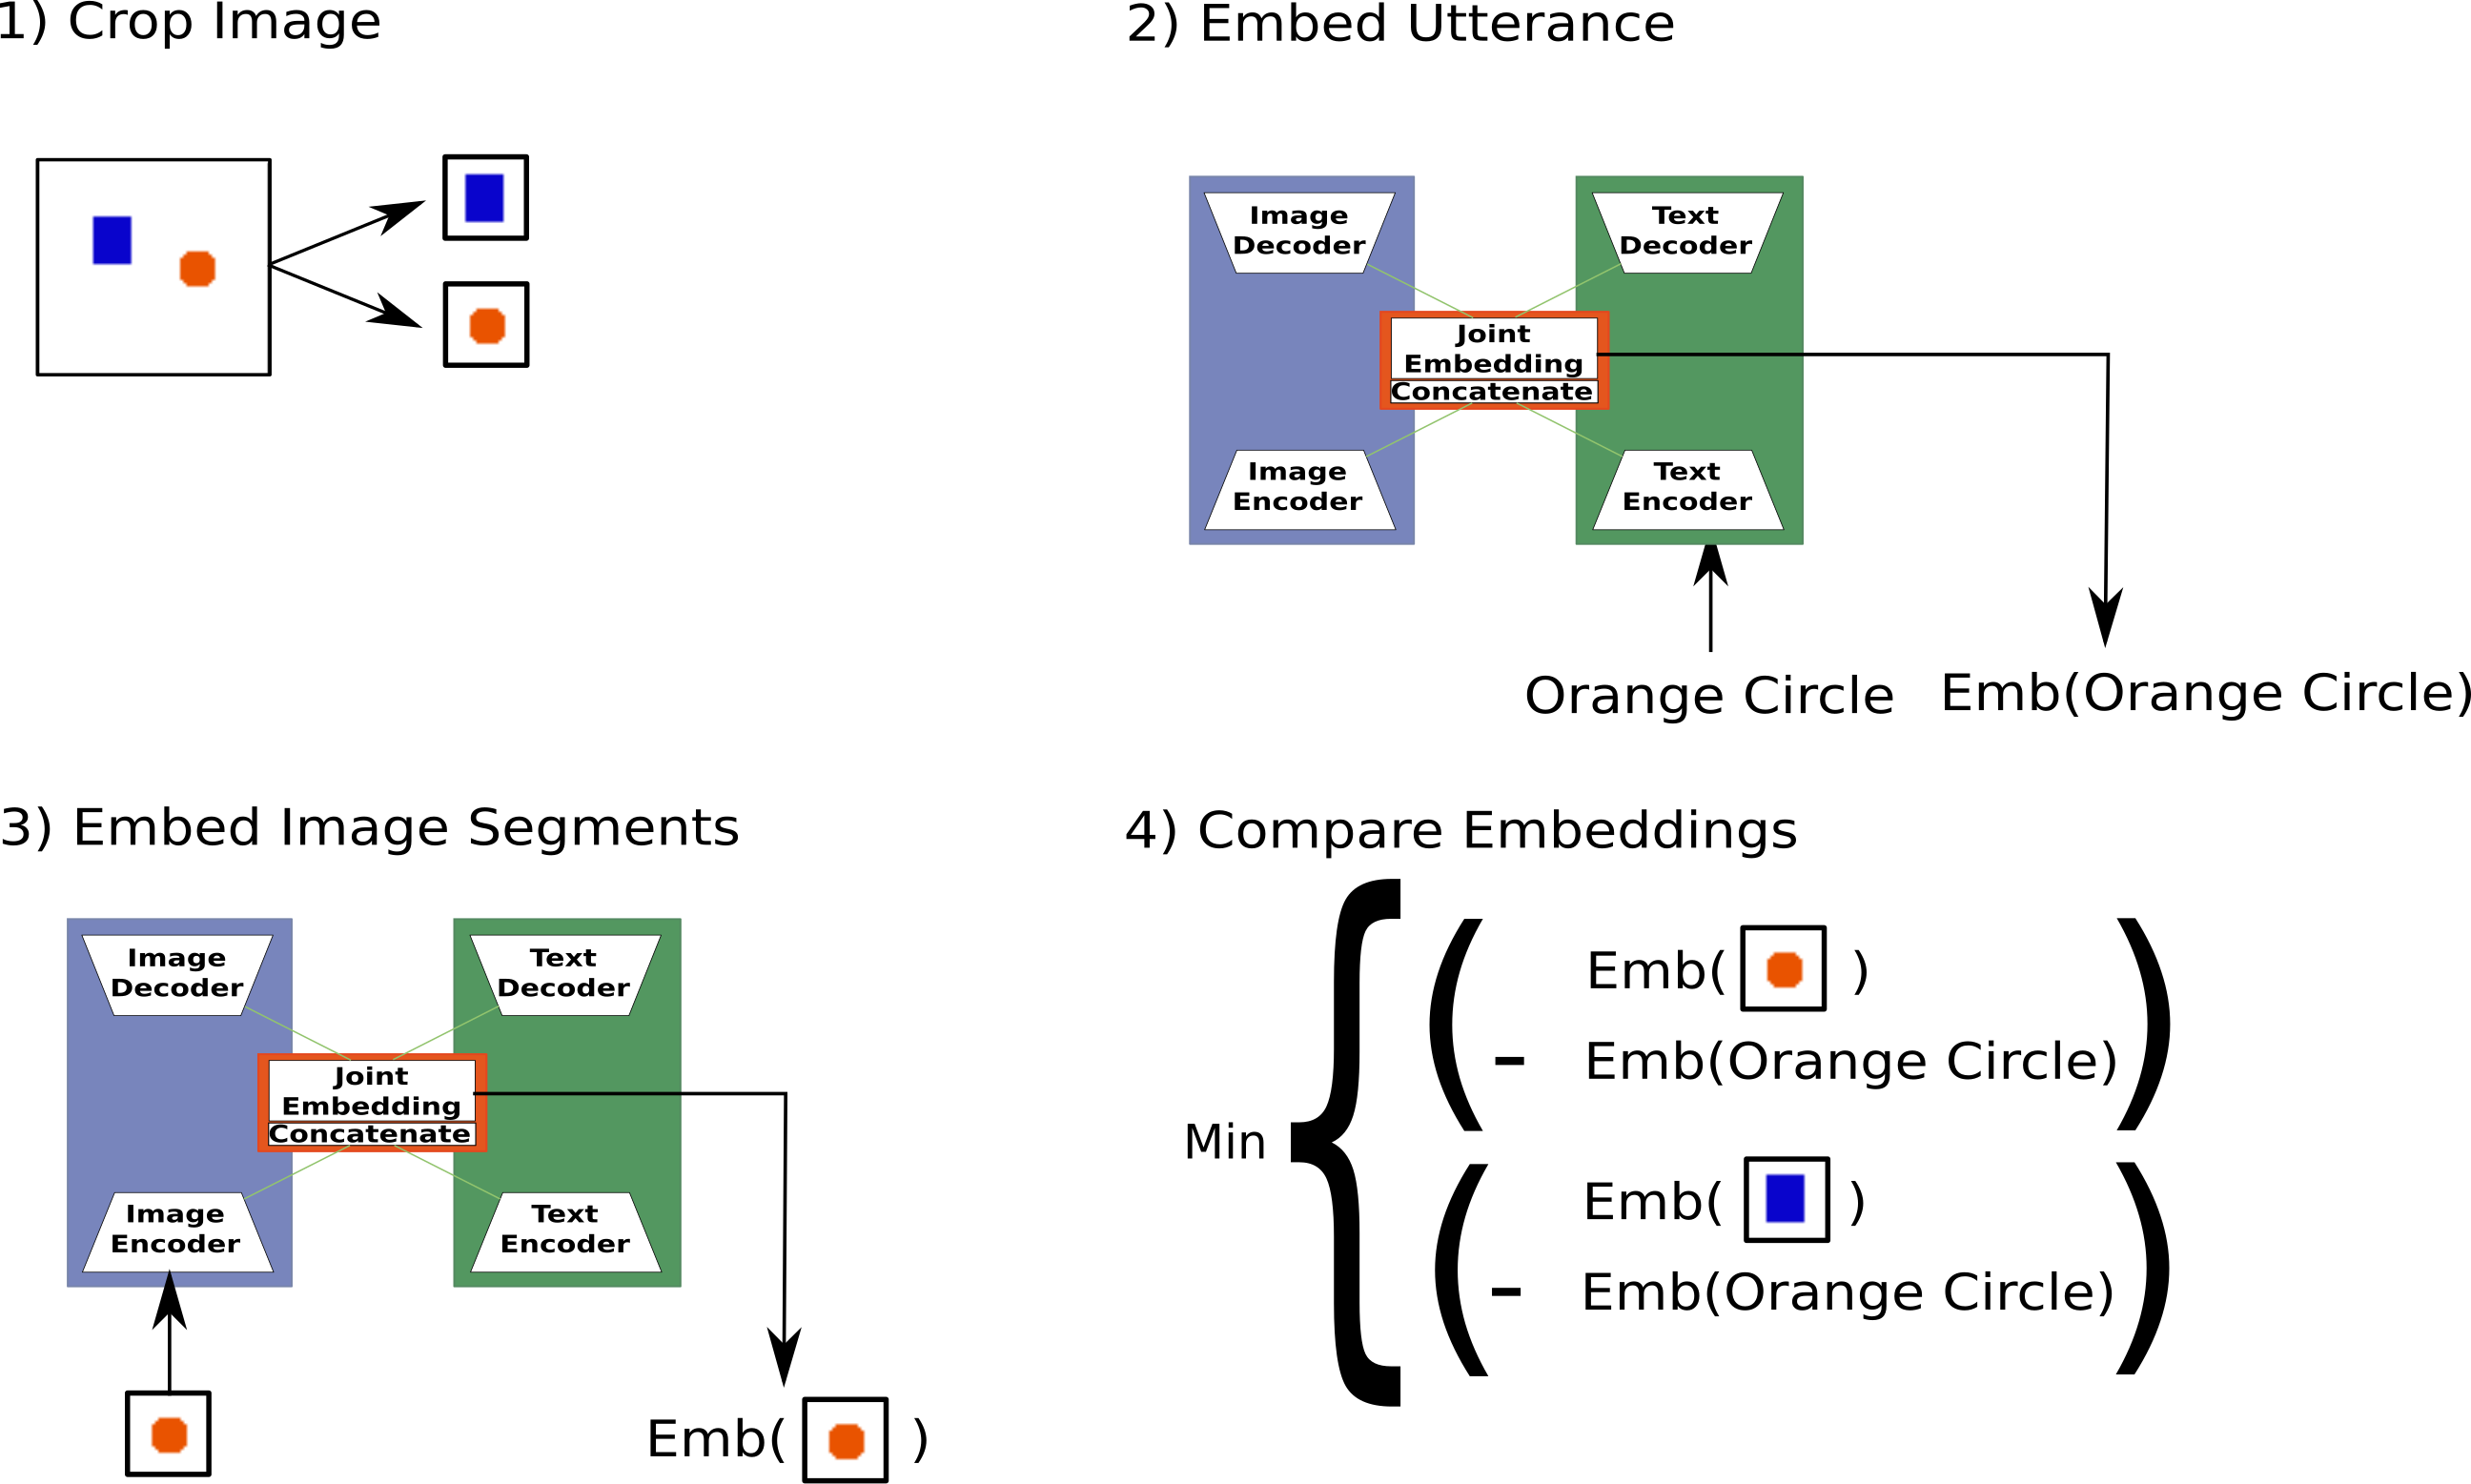
\includegraphics[width=\textwidth]{Figs/shapes/findingRefferant.png}
\caption{An example of using an MAE trained with MRL to disambiguate which object is being referred to in a scene.}
\label{fig:disamb}
\end{figure}

First, the image is split into patches, this can be done naively by sliding a window over the image and processing each patch. However this is not very computationally efficient and is likely to give ambiguous results, depending on the stride of the window, as multiple image patches may contain parts of the object of interest. Therefore it would be sensible to make use of an object detector such as Yolo v3 \cite{redmon2018yolov3} to predict object bounding boxes.

Comparing the embedding of each image patch to the embedding of the query, the image patch of interest should have the smallest \ac{MSE} between it and the query.

In order for the scenario depicted in \autoref{fig:disamb}, an \ac{NLU} module must be trained to extract the Intent of the human's utterance as well as any Entities which the human refers to. Fortunately, these types of \acp{NLU} are easily built using open source libraries like Rasa \cite{rasa}.



Developing the infrastructure for this type of scenario would allow for the exploration of questions such as:

\begin{itemize}
\item How many training examples does the \ac{MAE} require to operate accurately?
\item Is their an upper limit on the number of objects, visual attributes and words which the \ac{MAE} can learn?
\item How does regenerating a missing modality affect classification accuracy? Can the embedding of the regnerated missing modality be exploited to enhance  multimodal recognition techniques?
\end{itemize}

I believe \ac{MRL} can be used as a general tool for facilitating \ac{HRI} experiments, with the \ac{MAE} providing a piece of a cognitive architecture which translates low level sensory percepts (vision) to high level symbols (language).



\subsection{General System Improvements}
\textcolor{red}{More general improvements which could be made to the \ac{MAE} system which I have presented include architectural changes to the network, changes to the training scheme and the extending system to have a concept of time.}

\subsubsection{Architectural Improvements}
\textcolor{red}{In \autoref{Chapter3} I presented a time line of the developments of \acp{ANN} since Alexnet \cite{krizhevsky2012imagenet} in 2012. The addition of some or all of these features could improve the quality of the representation learnt by the \ac{MAE}. For example the addition of residual connections \cite{he2016deep} would allow for the training of a deeper \ac{MAE} which could increase the capacity of the network, allowing it to learn a larger variety of objects and having a more completely explored latent representation, thus improving the smoothness of the representation and potentially getting closer to proving hypothesis 5. The addition of multiscale convolutions \cite{szegedy2015going} could allow for better representation of objects of different sizes.}

\subsubsection{Training Scheme Improvements}
\textcolor{red}{The work of Reed et al. \cite{reed2016generative} has demonstrated how \acp{GAN} can be used to genrate images from captions for a very large and diverse dataset. Their dataset was much larger than the ReShape dataset and their method did not need to make use of class exemplars to achieve good quality image generation. I therefore propose that in future, combining these two methods to create a \ac{MAE} \ac{GAN} could lead to a fruitious area of research.}

\textcolor{red}{The addition of a variational cost \cite{kingma2013auto} or vector quantisation \cite{wavenet} on the latent representation could improve the smoothness of the representation and should be investigated in future.}


\subsubsection{Accounting for time}
\textcolor{red}{Another way in which this system could be enhanced would to be to make use of recurrent encoders and decoders in the \ac{MAE} like those seen in \cite{gregor2015draw}. By allowing the \ac{MAE} to iteratively learn to represent data, it is posisble that a better representation of the data could be generated, which in turn would lead to better generation of images, text or sound. Further to this, such an extension might allow my approach to \ac{MRL} to be applied to time dependant problems like action or speech recognition.}


%-----------------------------------
%	SUBSECTION 1
%-----------------------------------


